\documentclass[runningheads]{llncs}
%
\usepackage[utf8]{inputenc}
\usepackage[cmex10,fleqn]{amsmath}
\usepackage{amsfonts,amssymb}
%%\usepackage{amsfonts,amssymb,amsthm}
\usepackage{graphicx}
\usepackage{color}
\usepackage{todonotes}
%%\usepackage{algorithm,algpseudocode}
\usepackage{algorithm}
\usepackage{algorithmic}
%%\usepackage{algcompatible}
\usepackage{subfig}
\usepackage{xspace}
\usepackage{etoolbox}
\usepackage{xcolor}
\usepackage{multirow}
\usepackage{subfig}
\setlength{\tabcolsep}{3pt}

\definecolor{pdfurlcolor}{rgb}{0,0,0.6}
\definecolor{pdfcitecolor}{rgb}{0,0.6,0}
\definecolor{pdflinkcolor}{rgb}{0.6,0,0}

\usepackage[colorlinks=true,citecolor=pdfcitecolor,urlcolor=pdfurlcolor,linkcolor=pdflinkcolor,pdfborder={0
	0 0}]{hyperref}
%%\usepackage[breaklinks]{hyperref}
%%\usepackage{subcaption}

\usepackage{tikz}
\usetikzlibrary{matrix,snakes, patterns, positioning, shapes, calc, intersections, arrows, fit}

\graphicspath{{./diagrams/}{./plots/}}

%%\theoremstyle{plain}
%%\newtheorem{lemma}{Lemma}
%%\newtheorem{theorem}{Theorem}
%%\newtheorem{proposition}{Proposition}
%%\newtheorem{corollary}{Corollary}
%%\newtheorem{definition}{Definition}

%%\DeclareMathOperator{\FRT}{FRT}
%%\newcommand{\heteroprioD}{{HeteroPrioDep}\xspace}
\newcommand{\tensor}[1]{\cal\textbf{#1}\xspace}
\newcommand{\ttrain}{{\it Tensor-Train}\xspace}


% Used for displaying a sample figure. If possible, figure files should
% be included in EPS format.
%
% If you use the hyperref package, please uncomment the following line
% to display URLs in blue roman font according to Springer's eBook style:
% \renewcommand\UrlFont{\color{blue}\rmfamily}

\begin{document}
%
\title{Parallel Algorithms for Tensor-Train Decomposition}
%%%%\title{Contribution Title\thanks{Supported by organization x.}}
%%%%%
%%%%%\titlerunning{Abbreviated paper title}
%%%%% If the paper title is too long for the running head, you can set
%%%%% an abbreviated paper title here
%%%%%
\author{}
\institute{}
%%%%\author{First Author\inst{1}\orcidID{0000-1111-2222-3333} \and
%%%%Second Author\inst{2,3}\orcidID{1111-2222-3333-4444} \and
%%%%Third Author\inst{3}\orcidID{2222--3333-4444-5555}}
%%%%%
%%%%\authorrunning{F. Author et al.}
%%%%% First names are abbreviated in the running head.
%%%%% If there are more than two authors, 'et al.' is used.
%%%%%
%%%%\institute{Princeton University, Princeton NJ 08544, USA \and
%%%%Springer Heidelberg, Tiergartenstr. 17, 69121 Heidelberg, Germany
%%%%\email{lncs@springer.com}\\
%%%%\url{http://www.springer.com/gp/computer-science/lncs} \and
%%%%ABC Institute, Rupert-Karls-University Heidelberg, Heidelberg, Germany\\
%%%%\email{\{abc,lncs\}@uni-heidelberg.de}}
%%%%%
\maketitle       % typeset the header of the contribution

\begin{abstract}
The abstract should briefly summarize the contents of the paper in
150--250 words.

\keywords{First keyword \and Second keyword \and Another keyword.}
\end{abstract}

\section{Introduction}
\label{sec:introduction}
% 1-page
%%\begin{itemize}
%%	\item Popularity of tensors
%%	\item Need towards developing parallel and communication efficient algorithms
%%	\item HPC supercomputers
%%	\item tensor decomposition uses in Machine learning, Chemistry applications
%%	\item intuition behind Tensor train decomposition and its properties
%%	\item division of indices for TT and PTT decomposition
%%	\item outline of this paper
%%\end{itemize}
Multidimensional data are ubiquitous in scientific modeling. Tensors are becoming a popular choice in recent years to represent and manipulate such data. Tensor decomposition and approximation play important roles in several domains, for instance, quantum molecular dynamics, signal processing, numerical linear algebra, scientific simulations, data mining, neuroscience, computer vision, psychometrics, linguistics, chemometrics and more. Tensor decomposition based methods are also being used in drug discovery for the current pandemic~\cite{tensormethod-dd1,tensormethod-dd2}. We point the reader to~\cite{tensor-basics} for a nice survey on tensor decompositions and applications.
\todo[inline]{SK: Make smooth transition between paragraphs.}
Historically there has been a great emphasis on minmizing the complexity of computations. With the advent of multicores, the focus has shifted towards developing parallel algorithms. In recent years, the number of computational cores has increased drastically and communication becomes bottleneck for an application. Thus the focus is now moving towards developing parallel and communication optimal algorithms~\cite{qr-lu-2012,yelick2016,Ballard-mcnla-2011}.

Recent advances in high performance architectures make us enable to find efficient solutions for some of the most challenging scientific problems. Solving problems with large tensors on such architectures is still tough due to their large computational effort and memory requirements (amount of memory and computations grow exponentially in number of dimensions). These problems can not be tackled directly. It is therefore necessary to exploit patterns of the data. Finding low dimensional structure of high dimensional data is a powerful approach in this context. Several tensor representations such as CP, Tucker, Tensor-Train are based on low dimensional structure of the tensors. In this article, we concentrate on one of the tensor representations, namely, Tensor Train (TT). This representation and an algorithm to compute it were proposed recently in~\cite{tt}. It represents a $d$-dimensional tensor with $2$ matrices and $d$-$2$ 3-dimensional tensors. We call the algorithm TT-decomposition. The algorithm works in $d$-$1$ steps. In each step, one dimension is separated from the remaining tensor. Figure~\ref{fig:tt:ptt} illustrates graphical representation of the algorithm.

\begin{figure*}[htb]
	\begin{center}
		\includegraphics[scale=0.035]{./tt-ptt-decompositions.jpg}
		\caption{TT and PTT decompositions of a $d$-dimensional tensor~\label{fig:tt:ptt}.}
	\end{center}
\end{figure*}

\todo[inline]{SK: Explain intuition behind going from Figure~\ref{fig:tt:ptt}(a) to Figure~\ref{fig:tt:ptt}(b).}
TT-decomposition algorithm is sequential. As mentioned above, we are interested in parallel and communication optimal algorithms. In this article we propose a parallel algorithm to compute TT-representation of a tensor and we call it Parallel Tensor Train (PTT) decomposition throughout the text. Designing communication optimal algorithms to compute TT-representation of a tensor is a part of our future work. Our PTT decomposition algorithm divides the tensor into two subtensors at each level. It exposes parallelism in a binary tree shape. It has maximum parallelism at the last level of the tree. Figure~\ref{fig:tt:ptt} shows the splitting of a $d$-dimensional tensor into substensors by this algorithm. We prove that the ranks of TT-representation computed by this algorithm are bounded by the ranks of unfolding matrices of the tensor. We propose several heuristics to compute approximation of a tensor in TT-format and evaluate them for different tensor sizes. Here are the main contributions of this paper:
\begin{itemize}
	\item Propose a parallel algorithm PTT to compute TT-representation of a tensor
	\item Proof for bounded ranks of TT-representation obtained by PTT algorithm
	\item Different heuristics to obtain approximation of a tensor in TT-format
	\item Numerous experiments to assess the effectiveness of our heuristics for several low rank tensors and for tensors arising in molecular chemistry simulations 
\end{itemize}
  
\noindent The rest of the paper is organized as follows.



\section{Related Work}
\label{sec:relatedWork}
%0.5 page
\begin{itemize}
%%	\item Different types of tensor decompositions
%%	\item Properties and limitation of each type of tensor decomposition (Look at Osoledets's advisor work)
	\item Kolda's work
	\item Ballard's work (also include Communication-Efficient Parallel Algorithms forTensor Train Orthogonalization and Rounding)
	\item Solomonik's work
	\item Link between DMRG and Tensor-train
	\item Lin's work ~\cite{lin2019lowrank}
	\item Work on MTTKRP (Bora's work)
	\item May be: Vuduc's work, Sadayappan's work
	\item Ongoing work on TAMM (Tensor Algebra for Many body Methods)~\cite{Kowalski2014}
\end{itemize}

Tensor decomposition was first introduced by \emph{Hitchcock} in 1927~\cite{hitchcock-1927}. This decomposition is now known as canonical decomposition (CANDECOMP). It rediscovered several times, mainly in  psychometrics literature~\cite{redisover-candlecom-1,redisover-candlecom-2}. It can be viewed as high order generalization of singular value decomposition. CANDECOMP represents a $d$-dimensional tensor \tensor{A} with elements $A(i_1,\cdots,i_d)$ as: $A(i_1,\cdots,i_d) = \sum_{\alpha=1}^{r} U_1(i_1,\alpha)  U_2(i_2,\alpha)\cdots U_2(i_d,\alpha)$. The minimum number of $r$ required to express \tensor{A} is called the canonical rank. The matrices [$U_k(i_k,\alpha)$] are called canonical factors. The number of entries in the decoupled representation is $O(nrd)$, much less than the $O(n^d)$ entries in the original tensor. The most fascinating example of this decomposition in Algorithms is Strassen matrix multiplication, which  represents a $2 \times 2$ matrix multiplication as a decomposition of $4\times4\times4$ tensor~\cite{strassen-matrix-multiplication}. This decomposition suffers from several drawbacks. Determining the canonical rank of a tensor is an NP-complete problem~\cite{canonical-rank-npcomplete} and $3$ or higher dimensional tensors can fail to have best approximations for a fixed canonical rank~\cite{tensor-rank-best-low-rank-approximation}.

%%There is not any deterministic procedure to find the best approximation of a tensor for a fixed canonical rank.

\todo[inline]{SK: Not clear, Why Kolda is still using this decomposition? May be practical performance of some known algorithms is good.}

Another popular tensor decomposition is Tucker decomposition. It is named after Ledyard R. Tucker~\cite{tucker-decomposition}. This is also viewed as high order generalization of singular value decomposition. It decomposes a tensor into a set of matrices and a small core tensor. It is represented as: $A(i_1,\cdots,i_d) = \sum_{\alpha_1=1}^{r_1}\cdots\sum_{\alpha_d=1}^{r_d} g_{\alpha_1\cdots\alpha_d}U_1(i_1,\alpha_1)\cdots U_d(i_d, \alpha_d)$. Tucker approximations can be computed by several SVDs for auxiliary matrices. The approximation computed by HOSVD algorithm increases the error atmost by $\sqrt{d}$~\cite{hosvd-quasi-optimality}. For $r_1=r_2\cdots =r_d=r$, tucker approximations store $O(ndr+r^d)$ entries. As the number of entries in this format is exponential in the number of dimension. Thus it is suitable for small dimensions, but not for large dimensions.

\section{Tensor Train Decomposition}
\label{sec:tt}
% 0.5 page
\begin{itemize}
	\item Tensor train decomposition
	\item Complexity and its analysis
\end{itemize}

\noindent Some quantum molecular simulations require manipulating as high as 10 to 100 dimensional tensors. An efficient representation of a tensor with small number of variables provides opportunities to work with such high dimensional tensors. \ttrain decomposition is a popular way to obtain such a representation with few number of variables. It was proposed recently in ~\cite{tt} by \textit{Oseledets}. It represents a $d$-dimensional tensor with $2$ matrices and $d$-$2$ $3$-dimensional tensors. These are called cores of the TT-decomposition.

\begin{figure}
	\begin{center}

	\includegraphics[scale=0.05]{./tt_decomposition.jpg}
	\caption{\ttrain decomposition of a tensor. An entry of a $d$-dimensional tensor is computed by multiplying corresponding matrix (or row/column) of each tensor core, i.e., $A(i_1, i_2,\cdots, i_d) = G_1(i_1)G_2(i_2)\cdots G_d(i_d)$.\label{fig:ttdiagram}}
	\end{center}
\end{figure}

\noindent With TT-decomposition, a $d$-dimensional tensor $n_1 \times n_2 \times \cdots \times n_d$ is represented with cores $G_k$ of size $r_{k-1}\times n_k\times r_k$, $k=1,2,\cdots d$, $r_0=r_d=1$ and its elements satisfy the following expression:
\begin{align*}
A(i_1, i_2,\cdots ,i_d) &= \sum_{\alpha_0 = 1}^{r_0} \sum_{\alpha_1 = 1}^{r_1} \cdots \sum_{\alpha_d = 1}^{r_d} G_1(\alpha_0, i_1, \alpha_1) G_2(\alpha_1, i_2, \alpha_2)\cdots G_d(\alpha_{d-1}, i_1, \alpha_d)\\
&= \sum_{\alpha_1 = 1}^{r_1} \cdots \sum_{\alpha_{d-1} = 1}^{r_{d-1}} G_1(1, i_1, \alpha_1) G_2(\alpha_1, i_2, \alpha_2)\cdots G_d(\alpha_{d-1}, i_1, 1)
\end{align*}

\noindent Here $G_k(\alpha_{k-1}, i_k, \alpha_k)$ are the elements of $G_k$. Since $r_0=r_d=1$, hence $G_1$ and $G_d$ cores are matrices. Other cores are $3$-dimensional tensors.

\noindent Figure~\ref{fig:ttrainchain} exhibits that the above expression can also be represented graphically by a linear chain where sum over circle nodes (indices $\alpha_k$) are assumed to compute an entry of the tensor. This figure looks like a train, hence the \ttrain (TT) name is used for the decomposition. 

\begin{figure}[htb]
	\begin{center}
		\includegraphics[scale=0.05]{./chaintt.jpg}
		\caption{Chain representation of \ttrain decomposition.\label{fig:ttrainchain}}
	\end{center}
\end{figure}


Let $A(i_1,i_2,\cdots, i_d)$ denote the elements of a $d$-dimensional tensor \tensor{A}. The dimensions of \tensor{A} are $n_1 \times n_2 \times \cdots \times n_d$. The $k$-th unfolding matrix of tensor \tensor{A} is represented by $A_k$.

\begin{align*}
A_k &= A_k(i_1, i_2,\cdots, i_k; i_{k+1},\cdots ,i_d)
\end{align*}

\noindent The first $k$ indices represent the rows of $A_k$ and the last $d-k$ the columns of $A_k$. The size of this matrix is $(\prod_{l=1}^{k}n_l)\times(\prod_{l=k+1}^{d}n_l)$. The rank of this matrix is denoted by $r_k$. Let ($r_1, r_2,\cdots, r_{d-1}$) denote the rank of each unfolding matrix of tensor \tensor{A}.

%%\noindent \textit{Oseledets} proposed an algorithm to compute Tensor Train (TT) decomposition of a tensor in ~\cite{tt}. We also describe this in Algorithm~\ref{alg:tt_original}. 

\noindent \textit{Oseledets} presented an algorithm to compute Tensor Train (TT) decomposition of a tensor. Here we present the main idea of his algorithm. Let \tensor{A} be a $d$-dimensional tensor with dimensions $n_1 \times n_2 \times \cdots \times n_d$. His algorithm operates in $d-1$ steps. In each step, one dimension of the tensor is decoupled from the remaining dimensions using singular value decomposition. In the first step, \tensor{A} is represented as a matrix of size $n_1$ $\times$ $n_2 n_3 \cdots n_d$ and svd is computed for this matrix. The left singular vectors corresponding to nonzero singular values are the first core of TT-decomposition. In the second step, interaction with the first core and the second dimension are represented as rows of the matrix while other dimensions $n_3\cdots n_d$ represent the columns. Again svd is computed for this matrix and left singular vectors are rearranged to obtain the second core of TT-decomposition. This process is repeated for $d-1$ steps. Hence $d-1$ cores are obtained by this process. Remaining matrix, which represents the interaction with the $d-1$th core and $n_d$, constitutes the last core of the decomposition. This algorithm returns tensor cores $G_k(\alpha_{k-1}, n_k, \alpha_k) _{1\le k\le d}$ and also ensures that $\alpha_k \le r_k$. We refer the reader to the original paper for more details about this algorithm~\cite{tt}. 

%%%% We also describe this in Algorithm~\ref{alg:tt_original}. 
%%
%%
%%%%SK: todo: remove this algorithm and express this in words
%%\begin{algorithm}[htb]
%%	\caption{\label{alg:tt_original}TT decomposition (\textcolor{green}{sequential})}
%%	\begin{algorithmic}[1]
%%		\REQUIRE $d$-dimensional tensor \tensor{A} and ranks ($r_1, r_2,\cdots, r_{d-1}$) 
%%		\ENSURE Cores $G_k(\alpha_{k-1}, n_k, \alpha_k) _{1\le k\le d}$ of the TT-decomposition with $\alpha_k \le r_k$ and $\alpha_0 = \alpha_d=1$
%%		\STATE Temporary tensor $\tensor{C}=\tensor{A}$, $\alpha_0=1$
%%		\FOR{$k=1$ \TO $d-1$} 
%%		\STATE // matrix of size $\alpha_{k-1} n_k \times n_{k+1}\cdots n_d$
%%		\STATE $C$ = reshape($C, \alpha_{k-1} n_k$) 
%%		\STATE SVD: $C=U \Sigma V^\intercal$
%%		\STATE $\alpha_k=$ rank($\Sigma$)
%%		\STATE // first $\alpha_k$ columns of $U$
%%		%%		\COMMENT {Hello}
%%		\STATE $U_k = U(;1:\alpha_k)$
%%		\STATE Temporary $T =\Sigma V^\intercal$
%%		\STATE //first $\alpha_k$ rows of $T$
%%		\STATE $C= T(1:\alpha_k;)$
%%		\STATE $G_k$ = reshape($U_k, \alpha_{k-1}, n_k, \alpha_k$)
%%		\ENDFOR
%%		\STATE $G_d = C$, $\alpha_d=1$
%%		\RETURN tensor cores $G_k(\alpha_{k-1}, n_k, \alpha_k) _{1\le k\le d}$
%%	\end{algorithmic}
%%\end{algorithm}
%%
%%Algorithm~\ref{alg:tt_original} returns a TT decomposition of tensor \tensor{A}. It also ensures that $\alpha_k \le r_k$ $_{1\le k < d}$. We refer the reader to the original paper~\cite{tt} for more details about this algorithm. 

The \textit{Oseledets}'s TT-decomposition algorithm is sequential. It separates one dimension in each step and then operate on the remaining portion in the next step. Most modern computing platforms are composed of several number of nodes and cores. Hence running a sequential algorithm on these platforms may result in poor utilization of resources. In the next section, we propose a parallel algorithm to perform tensor train decomposition which exhibits $\frac{d}{2}$-level of parallelism. We also prove that the tensor cores $G_k(\beta_{k-1}, n_k, \beta_k) _{1\le k\le d}$ produced by our algorithm satisfy $\beta_k \le r_k$ $_{1\le k < d}$ property.
 
%%The original TT decomposition algorithm is sequential. In this article, we modify the original algorithm so that it can run efficiently in parallel. The description of the modified algorithm is presented in the next section.

\section{Parallel Tensor Train Decomposition}
\label{sec:tt_parallel}
% 2.5 pages
%%\begin{itemize}
%%%%	\item Different notations
%%%%	\item Parallel Tensor train algorithm and its proof
%%	\item Working principle with a matrix diagram and its reshape property
%%	\item Its generalization idea that we can break it from anywhere
%%\end{itemize}

The original indices of a tensor are called external indices, while the indices arise due to SVD are called internal indices. $nE$ and $nI$ denote the number of external and internal indices respectively of a tensor. A tensor with elements $A(\alpha, i_1, i_2, i_3, \beta)$ has $3$ external and $2$ internal indices. We also extend the definition of unfolding matrix to take internal indices into account. The $k$-th unfolding of tensor \tensor{A}, whose elements are $A(\alpha, i_1, i_2, \cdots,i_k, i_{k+1}, \cdots, \beta)$, is represented as,
%%\todo[inline]{SK: define a tensor for this $A_k$ representation}
\begin{align*}
A_k &= A_k(\alpha, i_1, i_2, \cdots, i_k; i_{k+1}\cdots, \beta)
\end{align*}
Here we consider all indices from the beginning to $i_{k}$ as the rows of $A_k$ and the remaining indices as the columns of $A_k$.
%%\todo[inline]{SK: make this function smooth for recursive calls}
\begin{algorithm}[htb]
	\caption{\label{alg:tt_parallel}TT-parallel (parallel Tensor Train Decomposition)}
	\begin{algorithmic}[1]
		\REQUIRE $d$-dimensional tensor \tensor{A} and ranks ($r_1, r_2,\cdots r_{d-1}$) 
		\ENSURE Cores $G_k(\alpha_{k-1}, n_k, \alpha_k) _{1\le k\le d}$ of the TT-decomposition with $\alpha_k \le r_k$ and $\alpha_0 = \alpha_d=1$
		\IF{$nE(\tensor{A})> $$1$} 
		\STATE Find the middle external index $k$
%%		\STATE $k=$mid-external-index(\tensor{A}) 
%%		\STATE $A_k =$ reshape(\tensor{A},k)
		\STATE Compute unfolding matrix $A_k$ 
		\STATE Compute SVD: $A_k = U \Sigma V^\intercal$
		\STATE $\alpha_k=$ rank($\Sigma$)
		\STATE Select diagonal matrices $X_k$, $S_k$ and $Y_k$ such that $X_kS_kY_k = \Sigma(1:\alpha_k; 1:\alpha_k)$\label{alg:line:xsy}
%%		\STATE // first $\alpha_k$ columns of $U$
		\STATE $\tensor{A}$$_{left}$ = Tensor($U(;1:\alpha_k)X_k$)
		\STATE list1 = TT-parallel($\tensor{A}$$_{left}$, ($r_1, r_2,\cdots r_{k-1}$) )
%%		\STATE Temporary $T =\Sigma V$
%%		\STATE //first $\alpha_k$ rows of $\Sigma V$
		\STATE $\tensor{A}$$_{right}$ = Tensor($Y_kV^\intercal(1:\alpha_k;)$)
		\STATE list2 = TT-parallel($\tensor{A}$$_{right}$, ($r_{k+1},\cdots r_{d-1}$))
		\RETURN \{list1, list2\}
%%		\ELSIF{$nE(\tensor{A})==$$1$ and $nI(\tensor{A})==$$1$} 
%%		\STATE $k=$ external-index(\tensor{A})
%%		\STATE if $k$ is the first index of $\tensor{A}$ then $\alpha_0=1$ else $\alpha_d = 1$
%%		\STATE $G_k = \tensor{A}$
%%		\RETURN $G_k$
		\ELSE 
		\STATE Find the external index $k$
		\IF {$k$ is the last index of \tensor{A}} 
		\STATE $\alpha_d = 1$
		\STATE $G_k = \tensor{A}$
		\RETURN $G_k$
		\ENDIF
		\IF {$k$ is the first index of \tensor{A}}
		\STATE $\alpha_0 = 1$
		\ENDIF
		\STATE Compute unfolding matrix $A_k$
		\STATE Update $A_k$, $A_k = A_kS_k$
		\STATE $G_k$ = Tensor($A_k$)
		\STATE return $G_k$
		\ENDIF
	\end{algorithmic}
\end{algorithm} 

Algorithm~\ref{alg:tt_parallel} is recursive and returns the tensor cores of a TT decomposition for tensor \tensor{A}. It is possible to work directly with unfolding matrices in the above algorithm, however for the ease of presentation, intermediate unfolding matrices are converted to tensors several times. We can also note that selection of $X_k$, $S_k$ and $Y_k$ are not specified in line number~\ref{alg:line:xsy}. All our proofs in this paper apply no matter how these are chosen. However, the practical performance of the compression algorithm, which is based on this algorithm, depends on the selection of these matrices. In Section~\ref{sec:expResults}, we compare three options: i) $X_k=S_k=I$, $Y_k = \Sigma(1:\alpha_k; 1:\alpha_k)$ ii) $X_k = Y_k = \Sigma(1:\alpha_k; 1:\alpha_k)^{1/2}$, $S_k = I$ iii) $X_k = Y_k = \Sigma(1:\alpha_k; 1:\alpha_k)$, $S_k = \Sigma(1:\alpha_k; 1:\alpha_k)^{-1} $. In most cases, third option is often the better choice.

This algorithm exposes parallelism in binary tree shape. It achieves maximum $\frac{d}{2}$-level of parallelism at the last level of the tree.
Figure~\ref{fig:4dindices} shows that how indices of a $6$-dimensional tensor are divided by this algorithm.

%%\todo[inline]{SK: Draw final diagrams in tikz/xfig}

\begin{figure}[htb]
	\begin{center}
		\includegraphics[scale=0.06]{./indices-partition.jpg}
	\end{center}
	\caption{\label{fig:4dindices} Partition of indices for a $6$-dimensional tensor by Algorithm~\ref{alg:tt_parallel}.} 
\end{figure}


\begin{figure}[htb]
	\begin{center}
		\includegraphics[scale=0.05]{./reshaping-6d.jpg}
	\end{center}
	\caption{Diagramatic representation of unfolding matrices at all non-leaf nodes for a $6$-dimensional tensor by Algorithm~\ref{alg:tt_parallel_approx}.\label{fig:ptt:reshaping}}
\end{figure}

\noindent Figure~\ref{fig:ptt:reshaping} illustrates the working tree of Algorithm~\ref{alg:tt_parallel_approx} for a $6$-dimensional tensor. It shows tensor at each node in its index form. Leaf nodes are assigned to the cores of TT representation. It also displays unfolding matrices for non-leaf nodes.

\noindent The proof on the bound of TT ranks obtained by Algorithm~\ref{alg:tt_parallel} is described in the following theorem.

\begin{theorem}
	If for each unfolding $A_k$ of a $d$-dimensional tensor \tensor{A}, $rank(A_k)=r_k$, then Algorithm~\ref{alg:tt_parallel} produces a decomposition with TT ranks not higher than $r_k$.
\end{theorem}
\begin{proof}
	Let us consider unfolding matrix $A_k$ of a $d$-dimensional tensor \tensor{A}. The rank of this matrix is $r_k$; hence it can be written as:
	\begin{align*}
	A_k &= U \Sigma V^\intercal\\
	A_k(i_1,i_2,\cdots,i_k;i_{k+1},\cdots, i_d) &= \sum_{\alpha=1}^{r_k} U(i_1,i_2,\cdots,i_k, \alpha)\Sigma(\alpha, \alpha)V(\alpha,i_{k+1},\cdots, i_d)\\
	&= \sum_{\alpha=1}^{r_k} U(i_1,i_2,\cdots,i_k, \alpha)X(\alpha, \alpha)S(\alpha, \alpha)Y(\alpha, \alpha)V(\alpha,i_{k+1},\cdots, i_d)\\
	&= \sum_{\alpha=1}^{r_k} B(i_1,i_2,\cdots,i_k, \alpha)S(\alpha, \alpha)C(\alpha,i_{k+1},\cdots, i_d)\\
	A_k &= BSC^\intercal
	\end{align*}	
%%	\begin{align*}
%%	U &= A_k V(V^\intercal V)^{-1} = A_k X\\
%%	V &= A_k^\intercal U(U^\intercal U)^{-1} = A_k^T W
%%	\end{align*}

	\begin{align*}
%%	\begin{center}
B = A_k (C^\intercal)^{-1}S^{-1} &= A_kZ\\
C = A_k^\intercal (B^\intercal)^{-1}S^{-1} &= A_k^\intercal W
%%	\end{center}
\end{align*}
	
	\noindent Or in the index form,
%%	\begin{align*}
%%	U(i_1,i_2,\cdots, i_k, \alpha) &= \sum_{i_{k+1}=1}^{n_{k+1}}\cdots\sum_{i_d=1}^{n_d} A(i_1, i_2, \cdots, i_d) X(\alpha, i_{k+1},\cdots, i_d)\\
%%	V(\alpha, i_{k+1},\cdots, i_d) &= \sum_{i_1=1}^{n_1} \cdots \sum_{i_k=k}^{n_k} A(i_1, i_2, \cdots, i_d) W(i_1,i_2,\cdots, i_k, \alpha)
%%	\end{align*}
	\begin{align*}
	B(i_1,i_2,\cdots, i_k, \alpha) &= \sum_{i_{k+1}=1}^{n_{k+1}}\cdots\sum_{i_d=1}^{n_d} A(i_1, i_2, \cdots, i_d) Z(\alpha, i_{k+1},\cdots, i_d)\\
	C(\alpha, i_{k+1},\cdots, i_d) &= \sum_{i_1=1}^{n_1} \cdots \sum_{i_k=k}^{n_k} A(i_1, i_2, \cdots, i_d) W(i_1,i_2,\cdots, i_k, \alpha)
	\end{align*}
	
	\noindent $B$ and $C$ can be treated as $k+1$ and $d-k+1$ dimensional tensors respectively. Now we consider unfolding matrices $B_1, B_2, \cdots, B_{k-1}$ and $C_{k+1},\cdots, C_{d-1}$ of $B$ and $C$. We will show that rank($B_{k'}$)$ \le r_{k'}$ $_{1\le k' \le k-1}$ and rank($C_{k'}$)$\le r_{k'}$ $_{k+1\le k' \le d-1}$.
	
	\noindent The rank of $A_{k'}$ is $r_{k'}$. Therefore, it can be represented as,
	\begin{align*}
	A(i_1, i_2, \cdots, i_d) &= \sum_{\beta=1}^{r_{k'}} F(i_1,i_2,\cdots ,i_{k'}, \beta) G(\beta, i_{k'+1},\cdots, i_d)
	\end{align*}
	Now, 
	\begin{align*}
	B_{k'} &= B(i_1,i_2, \cdots, i_{k'}; i_{k'+1},\cdots,i_k, \alpha)\\
	&= \sum_{i_{k+1}=1}^{n_{k+1}}\cdots\sum_{i_d=1}^{n_d} A(i_1, i_2, \cdots, i_d)Z(\alpha, i_{k+1},\cdots, i_d)\\
	&= \sum_{\beta=1}^{r_{k'}} \sum_{i_{k+1}=1}^{n_{k+1}}\cdots\sum_{i_d=1}^{n_d} F(i_1,i_2,\cdots ,i_{k'}, \beta) G(\beta, i_{k'+1},\cdots, i_d) Z(\alpha, i_{k+1},\cdots, i_d)\\
	&= \sum_{\beta=1}^{r_{k'}} F(i_1,i_2,\cdots ,i_{k'}, \beta) H(\beta,i_{k'+1},\cdots, i_k, \alpha)
	\end{align*}
	\noindent where,
	\begin{align*}
	H(\beta,i_{k'+1},\cdots, i_k, \alpha) =& \sum_{i_{k+1}=1}^{n_{k+1}}\cdots\sum_{i_d=1}^{n_d} G(\beta, i_{k'+1},\cdots, i_d) Z(\alpha, i_{k+1},\cdots, i_d)
	\end{align*}
	\noindent Row and column indices of $B_{k'}$ are now separated. Hence rank($B_{k'}$)$ \le r_{k'}$.
	
	\medskip
	\noindent Similarly for $C_{k'}$,
	\begin{align*}
	C_{k'}&= C(\alpha, i_{k+1}, \cdots, i_{k'}; i_{k'+1},\cdots, i_d)\\
	&= \sum_{i_1=1}^{n_1} \cdots \sum_{i_k=k}^{n_k} A(i_1, i_2, \cdots, i_d) W(i_1,i_2,\cdots, i_k, \alpha)\\
	&= \sum_{\beta=1}^{r_{k'}} \sum_{i_1=1}^{n_1} \cdots \sum_{i_k=k}^{n_k} F(i_1,i_2,\cdots ,i_{k'}, \beta) G(\beta, i_{k'+1},\cdots, i_d) W(i_1,i_2,\cdots, i_k, \alpha)\\ 
	&= \sum_{\beta=1}^{r_{k'}} M(\alpha, i_{k+1}, \cdots, i_{k'}, \beta) G(\beta, i_{k'+1},\cdots, i_d)
	\end{align*}	
	\noindent where
	\begin{align*}
	M(\alpha, i_{k+1}, \cdots, i_{k'}, \beta) &= \sum_{i_1=1}^{n_1} \cdots \sum_{i_k=k}^{n_k} F(i_1,i_2,\cdots ,i_{k'}, \beta) W(i_1,i_2,\cdots, i_k, \alpha)
	\end{align*}
	\noindent Here also row and column indices of $C_{k'}$ are separated. Hence rank($C_{k'}$)$ \le r_{k'}$.
	
	%%	This process continues recursively until each subtensor has exactly one external index. 
	When Algorithm~\ref{alg:tt_parallel} terminates, we have a list of tensors with exactly one external index. These tensors are cores of a TT-representation. As the above proof holds for each recursive partition, hence TT ranks of the decomposition produced by Algorithm~\ref{alg:tt_parallel} are bounded by $r_k$. This completes the proof.
\end{proof}

\indent The above proof is independent of from which index we split tensors into two subtensors. However in Algorithm~\ref{alg:tt_parallel}, we split the tensor from the middle external index.


\section{Tensor Train Approximation and Our Heuristics}
\label{sec:heuristics}
% 1 page
%%\begin{itemize}
%%	\item Our heuristics
%%	\item different performance metrics
%%\end{itemize}

%%Tensor decompositions are often approximated with a controllable global error to cope with noise and numerical instability. In this section, we propose different heuristics such that the approximated tensor is close to the original tensor by some prescribed accuracy.

Tensor decompositions are often approximated to cope with noise and numerical instability. In practical computations, rank-$r_k$ approximation of a tensor or an approximated tensor with certain accuracy is desired. Algorithm~\ref{alg:tt_parallel} can be used to compute rank-$r_k$ approximation of a tensor instead of exact low-rank decomposition. However we are yet to claim any optimality on its approximation and it is a part of our future work.

We modify Algorithm~\ref{alg:tt_parallel} to compute an approximated tensor in TT-format that is close by the prescribed accuracy, and present it in Algorithm~\ref{alg:tt_parallel_approx}.
 
\begin{algorithm}[htb]
	\caption{\label{alg:tt_parallel_approx}TT-parallel-approx (parallel Tensor Train approximation)}
	\begin{algorithmic}[1]
		\REQUIRE $d$-dimensional tensor \tensor{A} and expected accuracy $\epsilon$ 
		\ENSURE Cores $G_k(\alpha_{k-1}, n_k, \alpha_k) _{1\le k\le d}$ of the approximated tensor $B$ in TT-format such that $||A-B||_F$ is close to or less than $\epsilon$
		\IF{$nE(\tensor{A})> $$1$} 
		\STATE Find the middle external index $k$
		\STATE Compute unfolding matrix $A_k$ 
		\STATE Compute SVD: $A_k = U \Sigma V^\intercal$
		\STATE Compute truncation\_accuracy $\delta$
		\STATE Compute $\alpha_k$ such that $A_k = U(;1:\alpha_k) \Sigma(1:\alpha_k; 1:\alpha_k) V^\intercal(1:\alpha_k;) + E_k$ and $||E_K||_F \le \delta$
		\STATE Select diagonal matrices $X_k$, $S_k$ and $Y_k$ such that $X_kS_kY_k = \Sigma(1:\alpha_k; 1:\alpha_k)$
		\STATE $\tensor{A}$$_{left}$ = Tensor($U(;1:\alpha_k)X_k$)
		\STATE list1 = TT-parallel-approx($\tensor{A}$$_{left}$, $\epsilon_1$)
		\STATE $\tensor{A}$$_{right}$ = Tensor($Y_kV^\intercal(1:\alpha_k;)$)
		\STATE list2 = TT-parallel-approx($\tensor{A}$$_{right}$, $\epsilon_2$)
		\RETURN \{list1, list2\}
		\ELSE 
		\STATE Find the external index $k$
		\IF {$k$ is the last index of \tensor{A}} 
		\STATE $\alpha_d = 1$
		\STATE $G_k = \tensor{A}$
		\RETURN $G_k$
		\ENDIF
		\IF {$k$ is the first index of \tensor{A}}
		\STATE $\alpha_0 = 1$
		\ENDIF
		\STATE Compute unfolding matrix $A_k$
		\STATE Update $A_k$, $A_k = A_kS_k$
		\STATE $G_k$ = Tensor($A_k$)
		\STATE return $G_k$
		\ENDIF
	\end{algorithmic}
\end{algorithm}

Values of $\delta$, $\epsilon_1$ and $\epsilon_2$ in Algorithm~\ref{alg:tt_parallel_approx} depend on the selection of diagonal matrices $X_k$, $Y_k$ and $S_K$. We show in next subsection that how product of approximated matrices impact the accuracy of the result when applied with svd truncation. Based on the expression of next subsection, we compute $\epsilon_1$ and $\epsilon_2$ for different choices of $X_k$, $Y_k$ and $S_K$ in Section~\ref{sec:heuristics:all}. 


%%we propose different heuristics such that the approximated tensor is close to the original tensor by some prescribed accuracy. 
\subsection{Frobenius Error with Product of Approximated Matrices}
\label{sec:heuristics:approxproduct}

The following equation represents the singular value decomposition of a real matrix $A$.
\begin{equation*}
A=U\Sigma V^T
\end{equation*}

\noindent We can also write the above equation in the following way.
\begin{align*}
A&=(U_1 U_2)\begin{pmatrix}
\Sigma_1 & 0\\
0 & \Sigma_2
\end{pmatrix}(V_1 V_2)^T\\
&= U_1\Sigma_1 V_1^T + U_2 \Sigma_2 V_2^T\\
&= U_1\Sigma_1 V_1^T + E_A \\
&= BSC + E_A
\end{align*}

\noindent Here $B = U_1 X$, $C=YV_1^T$ and $XSY = \Sigma_1$. Matrices $B$ and $C$ are approximated to $\hat{B}$ and $\hat{C}$, i.e., $B = \hat{B} + E_B$ and $C = \hat{C} + E_C$. $X$, $Y$ and $S$ are diagonal matrices. $E_A$, $E_B$ and $E_C$ represent error matrices corresponding to low-rank approximation of $A$, $B$ and $C$.

\noindent Our goal is to find an expression for $||A - \hat{B} S \hat{C}||_F$ in terms of $||E_A||_F$, $||E_B||_F$ and $||E_C||_F$.

\begin{align*}
A - \hat{B} S \hat{C} &= A - (B-E_B)S(C-E_C)\\
&= A - BSC + BSE_C + E_BSC - E_BSE_C\\
&= E_A + BSE_C + E_BSC - E_BSE_C
\end{align*}
Now we take square of Frobenius norm on both sides,
\begin{align*}
||A - \hat{B} S \hat{C}||_F^2 =& ||E_A + BSE_C + E_BSC - E_BSE_C||_F^2 \\
=& ||E_A||_F^2 + ||BSE_C||_F^2 + ||E_BSC||_F^2 + ||E_BSE_C||_F^2 \\
& + 2\boldsymbol{<}E_A, BSE_C\boldsymbol{>}_F + 2<E_A, E_BSC>_F -2 <E_A, E_BSE_C>_F\\
& + 2 <BSE_C, E_BSC>_F -2 <BSE_C, E_BSE_C>_F - 2<E_BSC, E_BSE_C>_F
\end{align*}

\noindent Here $<P, Q>_F$ denotes frobenius inner product of matrices P and Q, and it is defined as: $<P, Q>_F = trace(P^TQ) = trace(PQ^T)$.

\noindent As $U$ and $V$ are othogonal matrices in singular value decomposition of $A$. Hence we obtain the following expressions:
\begin{align*}
U_1^TU_2 = 0 & \implies B^TE_A = 0 \implies <E_A, BSE_C>_F = 0\\
V_1^TV_2 = 0 & \implies CE_A^T = 0 \implies <E_A, E_BSC>_F = 0 
\end{align*}
After putting these values in $||A - \hat{B}S\hat{C}||_F^2$ expression, we get
\begin{align*}
||A - \hat{B} S \hat{C}||_F^2 =& ||E_A||_F^2 + ||BSE_C||_F^2 + ||E_BSC||_F^2 + ||E_BSE_C||_F^2 \\
& -2 <E_A, E_BSE_C>_F + 2 <BSE_C, E_BSC>_F\\
& -2 <BSE_C, E_BSE_C>_F - 2<E_BSC, E_BSE_C>_F
\end{align*}

\noindent In general, targeted error of any compression is very low, therefore we assume that any term involving more than one error matrix would be close to zero. With this assumption, the above equation can be written as

\begin{equation*}
%%\label{eq:approx}
||A - \hat{B} S \hat{C}||_F^2 \approx ||E_A||_F^2 + ||BSE_C||_F^2 + ||E_BSC||_F^2
\end{equation*}

\subsection{Different Heuristics}
\label{sec:heuristics:all}

It is immediate that the expression of the previous subsection can be applied for each unfolding of Algorithm~\ref{alg:tt_parallel_approx}. Similar to the approach of~\cite{tt}, we take $||E_{A_k}||_F \le \frac{\epsilon}{\sqrt{d-1}}$. Let $B$ and $C$ correspond to unfolding of $d_1$ and $d_2$ dimensional tensors and $d_1 + d_2 = d$. For simplicity, we assume $\frac{||E_B||_F^2}{d_1-1} = \frac{||E_C||_F^2}{d_2-1} = \delta^2$. This implies $\frac{\epsilon_1^2}{d_1-1} = \frac{\epsilon_2^2}{d_2-1} = \delta^2$.

\noindent Now we propose three heuristics such that overall error of approximation of Alogrithm~\ref{alg:tt_parallel_approx} is less than or close to $\epsilon$.
\begin{enumerate}
	\item \textit{H1}: Here we select $X = I$, $Y = \Sigma_1$ and $S = I$.	
	\begin{align*}
	||A - \hat{B} S \hat{C}||_F^2 &\approx ||E_A||_F^2 + ||U_1IIE_C||_F^2 + ||E_BI\Sigma_1V_1^T||_F^2 \\
	&\le \frac{\epsilon^2}{d-1} + ||E_C||_F^2 + ||E_B\Sigma_1||_F^2 \\
	\text{From Cauchy} & \text{-Schwarz inequality,}\\
	&\le \frac{\epsilon^2}{d-1} + ||E_C||_F^2 + ||E_B||_F^2 ||\Sigma_1||_F^2 \\
	&= \frac{\epsilon^2}{d-1} + \delta^2 (d_2-1)+ \delta^2 (d_1-1) trace(\Sigma_1^2)\le \epsilon^2.
	\end{align*}
	\noindent After simplifying this expression we obtain
	\begin{align*}
	\delta &\le \epsilon \sqrt{\frac{d-2}{(d-1) (d_2 -1 + (d_1-1) trace(\Sigma_1^2))}}.
	\end{align*}
	
	\item \textit{H2}: We choose $X=Y=\Sigma_1^{\frac{1}{2}}$ and $S=I$.
	
	\begin{align*}
	||A - \hat{B} S \hat{C}||_F^2 &\approx ||E_A||_F^2 + ||U_1 \Sigma_1^{\frac{1}{2}} IE_C||_F^2 + ||E_B I \Sigma_1^{\frac{1}{2}} V_1^T||_F^2 \\
	&\le \frac{\epsilon^2}{d-1} + ||\Sigma_1^{\frac{1}{2}} E_C||_F^2 + ||E_B \Sigma_1^{\frac{1}{2}}||_F^2 \\
	\text{From Cauchy} & \text{-Schwarz inequality,}\\
	&\le \frac{\epsilon^2}{d-1} + ||E_C||_F^2 ||\Sigma_1^{\frac{1}{2}}||_F^2 + ||E_B||_F^2 ||\Sigma_1^{\frac{1}{2}}||_F^2 \\
	&= \frac{\epsilon^2}{d-1} + \delta^2 (d_2-1) trace(\Sigma_1) + \delta^2 (d_1 -1) trace(\Sigma_1)\le \epsilon^2.
	\end{align*} 
	\noindent After simplifying this expression we obtain
	\begin{align*}
	\delta &\le \frac{\epsilon}{\sqrt{(d-1)trace(\Sigma_1)}}.
	\end{align*}
	
	\item \textit{H3}: We choose $X=Y=\Sigma_1$ and $S=\Sigma_1^{-1}$.
	\begin{align*}
	||A - \hat{B} S \hat{C}||_F^2 &\approx ||E_A||_F^2 + ||U_1\Sigma_1 \Sigma_1^{-1} E_C||_F^2 + ||E_B \Sigma_1^{-1} \Sigma_1 V_1^T||_F^2\\
	&\le \frac{\epsilon^2}{d-1} + ||E_C||_F^2 + ||E_B||_F^2 \\
	&= \frac{\epsilon^2}{d-1} + \delta^2 (d_2 -1) + \delta^2 (d_1-1) \le \epsilon^2
	\end{align*}
	\noindent After simplifying this expression we get
	\begin{align*}
	\delta &\le \frac{\epsilon}{\sqrt{d-1}}.
	\end{align*}	
\end{enumerate}

\subsection{Additional Heuristic}
We also consider the approximation algorithm proposed by \textit{Oseledets} in ~\cite{tt} for evaluation. This can be considered as a special case of Algorithm~\ref{alg:tt_parallel_approx}, where $X=S=I$, $Y=\Sigma_1$, and $k$ is the first left external index. In each step, left subtensor only has one external index and assigned to one of the cores of TT representation. This is a sequential algorithm. A uniform truncation of $\frac{\epsilon}{\sqrt{d-1}}$ is applied for each unfolding, which is equivalent to select $\epsilon_1=0$ and $\epsilon_2=\epsilon\sqrt{\frac{d_2-1}{d-1}}$. Approximation error of this algorithm is bounded by the sum of truncation applied for each unfolding. We refer the original paper~\cite{tt} for more details. We call this heuristic \textit{Oseledets Tensor Train Approximation} (OTTA).

\medskip

\noindent The following table summarizes all parameters of different heuristics for Algorithm~\ref{alg:tt_parallel_approx}. Let left and right subtensors are denoted by \tensor{B} and \tensor{C}, and have $d_1$ and $d_2$ external dimensions.

\begin{table}[htb]
\begin{tabular}{|c|c|c|c|c|}
	\hline
	Heuristic & Description & $\epsilon_{A_k}$ & $\epsilon_1$ & $\epsilon_2$\\ \hline
	H1 & $X = I$, $Y = \Sigma_1$, $S = I$ & $\frac{\epsilon}{\sqrt{d-1}}$ & $\epsilon \sqrt{\frac{(d-2)(d_1-1)}{(d-1) (d_2 -1 + (d_1-1) trace(\Sigma_1^2))}}$ & $\epsilon \sqrt{\frac{(d-2)(d_2-1)}{(d-1) (d_2 -1 + (d_1-1) trace(\Sigma_1^2))}}$\\ \hline
	H2 & $X=Y=\Sigma_1^{\frac{1}{2}}$, $S=I$ & $\frac{\epsilon}{\sqrt{d-1}}$ &
	$\epsilon\sqrt{\frac{d_1-1}{(d-1)trace(\Sigma_1)}}$ & $\epsilon\sqrt{\frac{d_2-1}{(d-1)trace(\Sigma_1)}}$\\ \hline
	H3 & $X=Y=\Sigma_1$, $S=\Sigma_1^{-1}$ & $\frac{\epsilon}{\sqrt{d-1}}$ &
	$\epsilon\sqrt{\frac{d_1-1}{d-1}}$ & $\epsilon\sqrt{\frac{d_2-1}{d-1}}$\\ \hline 
	OTTA & $X=I$, $Y=\Sigma_1$, $S=I$ & $\frac{\epsilon}{\sqrt{d-1}}$ &
	$0$ & $\epsilon\sqrt{\frac{d_2-1}{d-1}}$\\ \hline
\end{tabular}
\caption{Summary of all considered heuristics\label{tab:heuristics}.}
\end{table}
It is not hard to observe that svd truncation of $\frac{\epsilon}{\sqrt{d-1}}$ is used for each unfolding in \textit{H3}.


\section{Experimental Setup \& Results}
\label{sec:expResults}
%%We implement all our heuristics in MATLAB and run on our personal computers. 
Our all heuristics are designed to run in parallel, but to avoid parallel implementation challenges and to show effectiveness of our approaches we use Matlab to implement all the heuristics. We consider the tensors produced by the low rank functions of Table~\ref{tab:lowRankFunctions} for our evaluation. Such low rank functions arise in numerous applications and we refer to~\cite{lowRankFunctions,lowRankFunction-BM-2005,lowRankFunction-HKT-2005} for more details about these functions.

\begin{table}[htb]
	\centering
	\begin{tabular}{|l|c|}
		\hline
		Log & $\log(\sum_{j=1}^{N}j i_j)$\\ \hline
		Sin & $\sin(\sum_{j=1}^{N}i_j)$\\ \hline
		Inverse-Square-Root (\textit{ISR}) & $\frac{1}{\sqrt{\sum_{j=1}^{N}i_j^2}}$\\ \hline
		Inverse-Cube-Root (\textit{ICR}) & $\frac{1}{\sqrt[3]{\sum_{j=1}^{N}i_j^3}}$\\ \hline
		Inverse-Penta-Root (\textit{IPR}) & $\frac{1}{\sqrt[5]{\sum_{j=1}^{N}i_j^5}}$\\ \hline
	\end{tabular}
	\caption{Low rank functions.\label{tab:lowRankFunctions}}
\end{table}

\subsection{Performance Metrics}

Let $NE$ denote the number of entries in the original tensor. $ne_H$ and $ne_{min}$ represent the number of entries in the TT-representation produced by heuristic $H$ and the minimum number of entries in TT-representation among all considered heuristics. We consider the following performance metrics to assess heuristic $H$ for tensor \tensor{A}.
\begin{enumerate}
	\item compression ratio (\textit{compr}): This is defined as, $compr_H(A)$ = $\frac{NE(A)- ne_H(A)}{NE(A)}*100$ (higher values are better). A high value for this ratio indicates that the TT-representation produced by the heuristic has a few number of entries.
	\item ratio to minimal ($r$): This is defined as, $r_H(A) = \frac{ne_H(A)}{ne_{min}(A)}$ (lower values are better). This ratio is at least $1$ and a value close to $1$ indicates a well-suited heuristic which achieves good compression for the given tensor. 
\end{enumerate}

\noindent We also observe accuracy (\textit{OA}) of the approximation for the heuristic. If the cores of TT-representation produced by the heuristic correspond to tensor \tensor{B}, then $OA_H$(\tensor{A}) = $||\tensor{A}-\tensor{B}||_F$.


\subsection{Experimental Evaluation}
First we consider $N=12$ and $i_j \in \{1, 2, 3, 4\}$ for the functions of Table~\ref{tab:lowRankFunctions}. This configuration produces a $12$-dimensional tensor with $4^{12}$ elements for each low rank function. We perform comparison of all the considered heuristics for the target accuracies of $10^{-3}$ and $10^{-6}$ in Table~\ref{tab:dim-12}. 
\todo[inline]{SK: Change $e-x$ to $\times 10^{-x}$ everywhere.}

\begin{table}[!htb]
	\centering
	\subfloat[Prescribed accuracy = $10^{-3}$.\label{tab:dim-12-accr-10-3}]{
		\begin{tabular}{|c|c|c|c|c|c|c|}
			%%		\toprule
			\hline
			Heuristic & Metric & Log & Sin & ISR & ICR & IPR\\ \hline
			\multirow{3}{*}{OTTA} & compr & 99.996 & 99.999 & 99.994 & 99.991 & 99.986 \\ \cline{2-7} 
			& ne & 596 & 176 & 992 & 1580 & 2336 \\ \cline{2-7} 
			& OA & 3.692e-04 & 2.615e-09 & 3.224e-04 & 4.233e-04 & 4.774e-04 \\ \cline{1-7}
			\multirow{3}{*}{H1} & compr & 99.987 & 99.999 & 99.985 & 99.976 & 99.964 \\ \cline{2-7} 
			& ne    & 2108 & 176 & 2536 & 4096 & 5960 \\ \cline{2-7} 
			& OA    & 1.824e-03 & 1.393e-11 & 2.244e-04 & 1.672e-04 & 3.731e-04 \\ \cline{1-7} 
			\multirow{3}{*}{H2} & compr & 99.989 & 99.999 & 99.986 & 99.977 & 99.968 \\ \cline{2-7} 
			& ne    & 1832 & 176 & 2352 & 3840 & 5404 \\ \cline{2-7} 
			& OA    & 7.042e-05 & 6.144e-12 & 2.036e-04 & 6.097e-05 & 2.981e-04 \\ \cline{1-7} 
			\multirow{3}{*}{H3} & compr & 99.996 & 99.999 & 99.994 & 99.991 & 99.986 \\ \cline{2-7} 
			& ne    & 596 & 176 & 992 & 1528 & 2336 \\ \cline{2-7} 
			& OA    & 3.692e-04 & 1.252e-11 & 3.223e-04 & 5.042e-04 & 4.773e-04 \\ \cline{1-7}  
		\end{tabular}
	}

	\subfloat[Prescribed accuracy = $10^{-6}$.\label{tab:dim-12-accr-10-6}]{
	\begin{tabular}{|c|c|c|c|c|c|c|}
		%%		\toprule
		\hline
		Heuristic & Metric & Log & Sin & ISR & ICR & IPR\\ \hline
		\multirow{3}{*}{OTTA} & compr & 99.993 & 99.999 & 99.987 & 99.981 & 99.971 \\ \cline{2-7} 
		& ne    & 1212 & 176 & 2240 & 3184 & 4864 \\ \cline{2-7} 
		& OA    & 2.271e-07 & 2.615e-09 & 1.834e-07 & 4.884e-07 & 4.836e-07 \\ \cline{1-7} 
		\multirow{3}{*}{H1} & compr & 99.939 & 99.999 & 99.944 & 99.915 & 99.873 \\ \cline{2-7} 
		& ne    & 10268 & 176 & 9312 & 14224 & 21308 \\ \cline{2-7} 
		& OA    & 8.959e-07 & 1.393e-11 & 1.404e-07 & 9.258e-08 & 1.249e-07 \\ \cline{1-7} 
		\multirow{3}{*}{H2} & compr & 99.799 & 99.999 & 99.952 & 99.912 & 99.870 \\ \cline{2-7} 
		& ne    & 33772 & 176 & 8068 & 14824 & 21792 \\ \cline{2-7} 
		& OA    & 2.820e-08 & 6.144e-12 & 1.118e-07 & 8.518e-08 & 5.664e-08 \\ \cline{1-7} 
		\multirow{3}{*}{H3} & compr & 99.993 & 99.999 & 99.987 & 99.981 & 99.970 \\ \cline{2-7} 
		& ne    & 1212 & 176 & 2240 & 3184 & 4964 \\ \cline{2-7} 
		& OA    & 2.265e-07 & 1.252e-11 & 1.834e-07 & 4.884e-07 & 3.999e-07 \\ \cline{1-7}   
	\end{tabular}
    }
	\caption{Comparison of different heuristics for $12$-dimensional tensors.\label{tab:dim-12}}
\end{table}

%%\todo[inline]{SK: Explain details of Table~\ref{tab:dim-12}.}
\noindent Table~\ref{tab:dim-12-accr-10-3} shows comparable compression ratios for all heuristics. $H2$ achieves slightly better compression ratios than $H1$. $H3$ compression ratios are best among all our heuristics and are also almost equal or better than $OTTA$. We can also observe that $ne$ values of ICR function are more than ISR function and less than IPR function. This indicates that the low-rank approximation of function $(\sum_j i_j^p)^\frac{1}{p}$ requires more entries as $p$ increases. $OA$ values of all heuristics are also within or close to the prescribed accuracy.

%%except for the $H1$ heuristic with $Log$ function.
\todo[inline]{SK: Find the exact term due to which $OA$ value of $H1$ heuristic with $Log$ function is more than the prescribed limit.}

\noindent Table~\ref{tab:dim-12-accr-10-6} also shows similar behavior. $H3$ compression ratios are best among all our heuristics and are similar to $OTTA$. $OA$ values of all heuristics are also within the prescribed limit of $10^{-6}$. 
  
\noindent Next we take $N=6$ and $i_j \in \{1,2 \cdots ,16\}$ for the functions of Table~\ref{tab:lowRankFunctions}. This configuration produces a $6$-dimensional tensor with $16^6$ elements for each function. We present our performance metrics of all the considered heuristics for these tensors in Table~\ref{tab:dim-6}.

%%\todo[inline]{SK: Explain details of Table~\ref{tab:dim-6}.}
%% 4.206e-10 $ 4.206e-10$ $4.206 10^{-10}$ $4.206 \times 10^{-10}$
\begin{table}[!htb]
	\centering
	\subfloat[Prescribed accuracy = $10^{-3}$.\label{tab:dim-6-accr-10-3}]{
		\begin{tabular}{|c|c|c|c|c|c|c|}
			%%		\toprule
			\hline
			Heuristic & Metric & Log & Sin & ISR & ICR & IPR\\ \hline
			\multirow{3}{*}{OTTA} & compr & 99.987 & 99.998 & 99.976 & 99.962 & 99.928 \\ \cline{2-7} 
			& ne    & 2112 & 320 & 4064 & 6368 & 12032 \\ \cline{2-7} 
			& OA    & 2.831e-04 & 4.206e-10 & 4.587e-04 & 6.149e-04 & 4.429e-04 \\ \cline{1-7} 
			\multirow{3}{*}{H1} & compr & 99.953 & 99.998 & 99.948 & 99.920 & 99.867 \\ \cline{2-7} 
			& ne    & 7904 & 320 & 8736 & 13472 & 22240 \\ \cline{2-7} 
			& OA    & 7.578e-05 & 3.410e-12 & 2.080e-04 & 2.906e-04 & 2.268e-04 \\ \cline{1-7} 
			\multirow{3}{*}{H2} & compr & 99.973 & 99.998 & 99.952 & 99.928 & 99.879 \\ \cline{2-7} 
			& ne    & 4512 & 320 & 8096 & 12016 & 20288 \\ \cline{2-7} 
			& OA    & 7.268e-05 & 3.486e-12 & 2.033e-04 & 2.882e-04 & 2.218e-04 \\ \cline{1-7} 
			\multirow{3}{*}{H3} & compr & 99.987 & 99.998 & 99.976 & 99.962 & 99.928 \\ \cline{2-7} 
			& ne    & 2112 & 320 & 4064 & 6368 & 12032 \\ \cline{2-7} 
			& OA    & 2.832e-04 & 4.409e-12 & 4.588e-04 & 6.150e-04 & 4.430e-04 \\ \cline{1-7}  
		\end{tabular}
	}
	
	\subfloat[Prescribed accuracy = $10^{-6}$.\label{tab:dim-6-accr-10-6}]{
		\begin{tabular}{|c|c|c|c|c|c|c|}
			%%		\toprule
			\hline
			Heuristic & Metric & Log & Sin & ISR & ICR & IPR\\ \hline
			\multirow{3}{*}{OTTA} & compr & 99.974 & 99.998 & 99.945 & 99.915 & 99.845 \\ \cline{2-7} 
			& ne    & 4320 & 320 & 9184 & 14336 & 26048 \\ \cline{2-7} 
			& OA    & 4.156e-07 & 4.206e-10 & 3.990e-07 & 6.983e-07 & 4.536e-07 \\ \cline{1-7} 
			\multirow{3}{*}{H1} & compr & 99.740 & 99.998 & 99.841 & 99.783 & 99.696 \\ \cline{2-7} 
			& ne    & 43616 & 320 & 26688 & 36352 & 50976 \\ \cline{2-7} 
			& OA    & 1.147e-06 & 3.410e-12 & 2.841e-07 & 1.610e-07 & 1.958e-07 \\ \cline{1-7} 
			\multirow{3}{*}{H2} & compr & 99.824 & 99.998 & 99.902 & 99.854 & 99.772 \\ \cline{2-7} 
			& ne    & 29456 & 320 & 16416 & 24576 & 38208 \\ \cline{2-7} 
			& OA    & 3.584e-07 & 3.486e-12 & 2.822e-07 & 1.522e-07 & 1.802e-07 \\ \cline{1-7} 
			\multirow{3}{*}{H3} & compr & 99.974 & 99.998 & 99.945 & 99.915 & 99.845 \\ \cline{2-7} 
			& ne    & 4320 & 320 & 9184 & 14336 & 26048 \\ \cline{2-7} 
			& OA    & 4.156e-07 & 4.409e-12 & 3.990e-07 & 6.985e-07 & 4.538e-07 \\ \cline{1-7}   
		\end{tabular}
	}
	\caption{Comparison of different heuristics for $6$-dimensional tensors.\label{tab:dim-6}}
\end{table}


\noindent Table~\ref{tab:dim-6} displays comparable compression ratios for all heuristics. Again $H3$ compression ratios are best among all our heuristics and are same as $OTTA$. $OA$ values of all heuristics are also within or close to the prescribed accuracy. Decay of singular values for $Sin$ function is quite steep, hence performance metrics for both prescribed accuracies depict the same numbers. Sin (resp. IPR) function achieves the best (resp. worst) compression ratios among all the low rank functions of Table~\ref{tab:lowRankFunctions}.
  
\begin{figure}[!htb]
	\begin{center}
		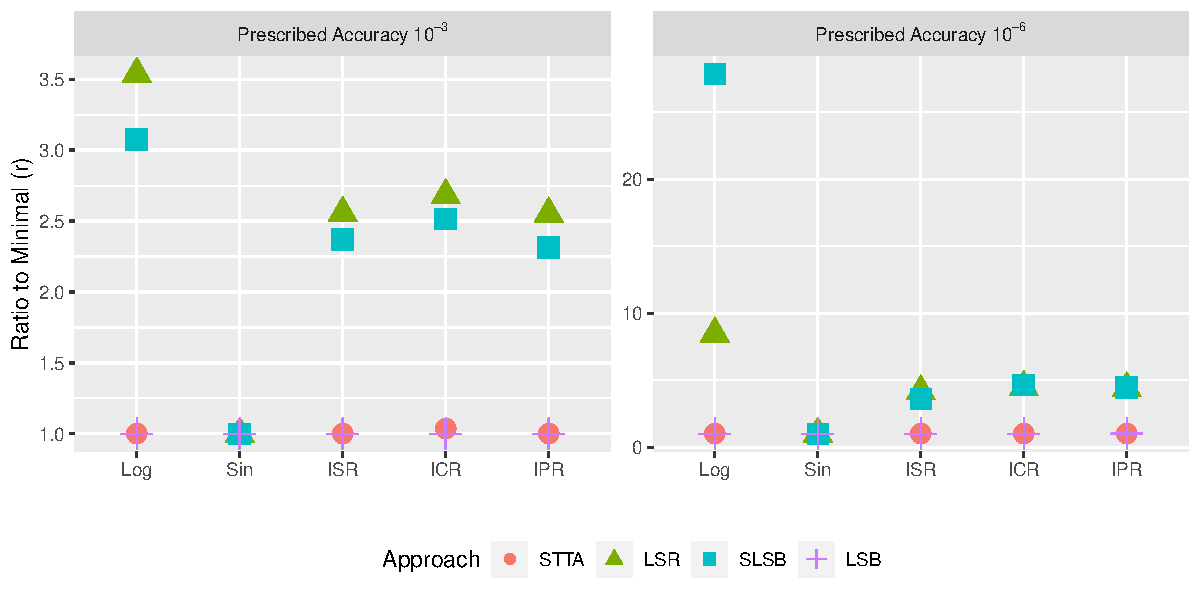
\includegraphics[scale=0.56]{./ratio_to_minimal-4-12.pdf}
	\end{center}
\caption{Comparison of ratio to minimal for $12$-dimensional tensors.\label{fig:rtm-12}}
\end{figure}

\noindent Figure~\ref{fig:rtm-12} depicts $r$ values of all the considered heuristics for 12-dimensional tensors. All heuristics achieve the same compression ratio for $Sin$ function, hence $r$ values are $1$. $r_{H3}$ and $r_{OTTA}$ values are almost same and are equal to $1$. For the prescribed accuracy of $10^{-3}$, $r_{H1}$ values are between $2.5$ to $3.6$ for the other functions. $H2$ compression ratios are slightly better than $H1$, hence $r_{H2}$ values are smaller than $r_{H1}$, but still in the range of $2.25$ to $3.25$. For the prescribed accuracy of $10^{-6}$, $r_{H1}$ value for Log function is more than $25$. This indicates that $H1$ stores $25\times$ more entries than the best heuristic. $r_{H1}$ and $r_{H2}$ are similar for ISR, ICR and IPR functions and are close to $5$. 

\begin{figure}[!htb]
	\begin{center}
		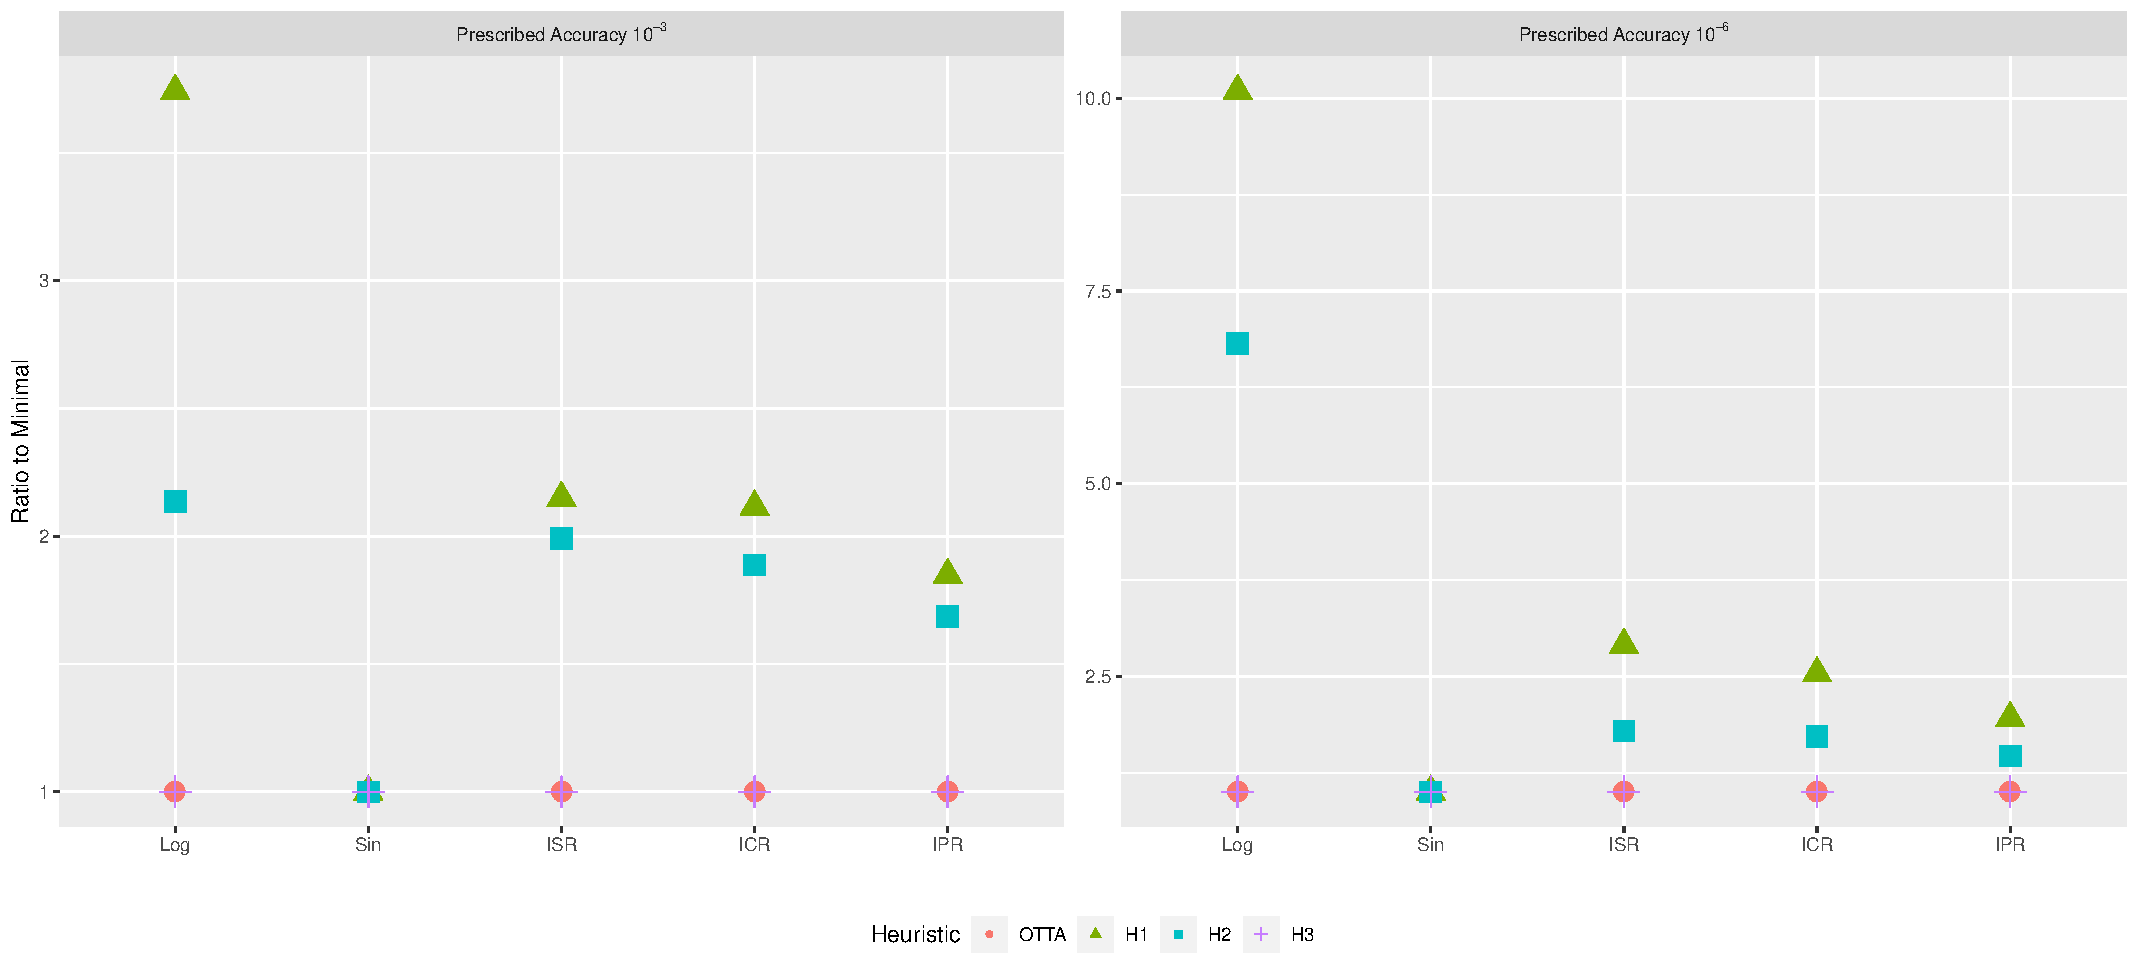
\includegraphics[scale=0.56]{./ratio_to_minimal-16-6.pdf}
	\end{center}
	\caption{Comparison of ratio to minimal for $6$-dimensional tensors.\label{fig:rtm-6}}
\end{figure}
%%Ratio to minimal values of the heuristics for $6$- dimensional tensors are shown in Figure~\ref{fig:rtm-6}.

\noindent Figure~\ref{fig:rtm-6} shows $r$ values of the heuristics for $6$-dimensional tensors. Similar to the previous plot, $r$ values of all heuristics for Sin function are $1$. ${H3}$ and ${OTTA}$ achieve similar compression, hence their values are equal and close to $1$. For the prescribed accuracy of $10^{-3}$, $r_{H1}$ value of Log function is more than $3.5$. Therefore $H1$ requires $3\times$ more storage than the best heuristic for this function. For other functions, its values are between $1.75$ to $2.25$. $r_{H2}$ values are slightly better than $r_{H1}$, and are in the range of $1.75$-$2.25$. For the prescribed accuracy of $10^{-6}$, $H1$ and $H2$ require $10\times$ and $6\times$ more storage than the best heuristic for Log function. $H1$ and $H2$ achieve close compression ratios for ISR, ICR and IPR functions. Hence their $r$ values are also close.

\medskip
\noindent From the results of this section, we notice that $OA$ values of $H2$ and $H3$ are always within the prescribed accuracy. We also observe that $H3$ achieves the best compression ratios among all our heuristics. 

\subsection{Evaluation for Molecular Chemistry Data}
%%As we observe in previous tables, 
As $H3$ is the best among all our proposed heuristics, we will consider only $OTTA$ and $H3$ for comparison in this section. We evaluate these heuristics for tensors arising in molecular chemistry simulations. These tensors correspond to interactions between electrons of different orbitals (and virtual orbitals), and are obtained by choosing different basis sets of $H_2O$, $H_2$ and $CH_4$ molecules. The obtained tensors are $4$-dimensional and have distinct sizes. Table~\ref{tab:dim-4-mol-chem} shows values of performance metrics for these tensors. Exp1, Exp2 and Exp3 correspond to simulations with $H_2O$ molecule, while Exp4 and Exp5 correspond to simulations with $H_2$ and $CH_4$ respectively. 
 
%%Choose molecule 1:H2O 2:H2 3:CH42
%%Choose basis 1:STO-nG,2:cc-pVDZ1
%%Choose basis 1:STO-3G 2:STO-6G1

\begin{table}[!htb]
	\centering
	\subfloat[Prescribed accuracy = $10^{-3}$.\label{tab:dim-4-mol-chem-accr-10-3}]{
		\begin{tabular}{|c|c|c|c|c|c|c|c|}
			%%		\toprule
			\hline
			Heuristic & Metric & Exp1 & Exp2 & Exp3 & Exp4 & Exp5 & Exp6\\ \cline{2-8}
%%			&& 1-1-1 & 1-1-2 & 1-2 & 2-1-1 & 2-2 & 3-1\\ \cline{2-8}
			& NE & $7^4$ & $7^4$ & $25^4$ & $2^4$ & $10^4$ & $35^4$\\ \hline
			\multirow{3}{*}{OTTA} & compr & 46.939 & 46.939 & 88.800 & -50.000 & 64.000 & 92.000\\ \cline{2-8}
			& ne    & 1274 & 1274 & 43750 & 24 & 3600 & 120050\\ \cline{2-8}
			& OA    & 1.969e-04 & 2.048e-04 & 4.819e-04 & 2.669e-04 & 2.536e-04 & 5.516e-04\\ \cline{1-8}
			\multirow{3}{*}{H3} & compr & 46.939 & 46.939 & 88.800 & -50.000 & 64.000 & 92.000\\ \cline{2-8}
			& ne    & 1274 & 1274 & 43750 & 24 & 3600 & 120050\\ \cline{2-8}
			& OA    & 1.969e-04 & 2.048e-04 & 4.819e-04 & 2.669e-04 & 2.536e-04 & 5.516e-04\\ \cline{1-8}  
		\end{tabular}
	}
	
	\subfloat[Prescribed accuracy = $10^{-6}$.\label{tab:dim-4-mol-chem-accr-10-6}]{
		\begin{tabular}{|c|c|c|c|c|c|c|c|}
			%%		\toprule
			\hline
			Heuristic & Metric & Exp1 & Exp2 & Exp3 & Exp4 & Exp5 & Exp6\\ \cline{2-8}
%%			&& 1-1-1 & 1-1-2 & 1-2 & 2-1-1 & 2-2 & 3-1\\ \cline{2-8}
			& NE & $7^4$ & $7^4$ & $25^4$ & $2^4$ & $10^4$ & $35^4$\\ \hline
			\multirow{3}{*}{OTTA} & compr & 6.122 & 2.041 & 73.760 & -100.000 & 32.000 & 78.775\\ \cline{2-8}
			& ne    & 2254 & 2352 & 102500 & 32 & 6800 & 318500\\ \cline{2-8}
			& OA    & 5.486e-07 & 1.073e-07 & 5.689e-07 & 5.940e-16 & 4.525e-07 & 5.521e-07\\ \cline{1-8}
			\multirow{3}{*}{H3} & compr & 6.122 & 2.041 & 73.760 & -100.000 & 32.000 & 78.775\\ \cline{2-8}
			& ne    & 2254 & 2352 & 102500 & 32 & 6800 & 318500\\ \cline{2-8}
			& OA    & 5.486e-07 & 1.073e-07 & 5.689e-07 & 5.057e-16 & 4.525e-07 & 5.521e-07\\ \cline{1-8}  
		\end{tabular}
	}
	\caption{Comparison of $OTTA$ and $H3$ for $4$-dimensional tensors generated from molecular chemistry simulations.\label{tab:dim-4-mol-chem}}
\end{table}

\noindent Table~\ref{tab:dim-4-mol-chem} shows that performance metrics of both heuristics are almost same. This behavior can be understand from the fact that for the considered tensors first and last cores of the approximated tensors have maximum number of entries. For instance, if $G_1$ and $G_4$ are the first and last cores of the approximation for the tensor of Exp3, then $G_1$ and $G_4$ both have $25\times25=625$ number of entries. The tensor obtained from Exp4 is very small and has only $16$ entries. TT-representation of the approximation of this tensor requires more than $16$ entries -- $24$ (resp. $32$) for the prescribed accuracy of $10^{-3}$ (resp. $10^{-6}$). For intermediate and large size tensors, both heuristics achieve very good compression ratios.
 
\section{Discussion}
\label{sec:discussion}
\begin{itemize}
	\item Implementation of first svd computation
	\item Complexity and storage of the extra buffer in H3 heuristic
	\item Other decomposition instead of svd
	\item Analysis of operations in both algorithms
\end{itemize}

\section{Conclusion}
\label{sec:conclusion}
\begin{itemize}
	\item Proof, heuristics and experiments
	\item Implementation of this approach
	\item RRQR instead of svd
	\item Combinatorial choices to find the best order to perform TT or PTT decomposition
\end{itemize}

%
% ---- Bibliography ----
%
% BibTeX users should specify bibliography style 'splncs04'.
% References will then be sorted and formatted in the correct style.
%
 \bibliographystyle{splncs04}
 \bibliography{paralleltt}

\end{document}
